\chapter{Theorie zur Signalverarbeitung}
\label{theorie}
%

Vor dem Einstieg in die Signalverarbeitung wird Hintergrundwissen benötigt. Für die Durchführung der Fourier Transform werden gleichzeitig aufgenommen Signale wieder in die ursprünglichen Signale getrennt. Die Komplexität erschließt sich durch die Darstellung vermischter Signale und dessen Schwierigkeit einzelne Signale wiederzufinden. Dafür werden zuvor der Aufbau einzelner Signalen behandelt, um zu erkennen wie Frequenzen dargestellt und abgelesen werden. 

%
\section{Was ist ein Ton?}
\label{sounds}
%

Töne entstehen durch die Vibrationen eines Gegenstandes, die Schallwellen erzeugen. Das Gehör kann diese Schwingungen der Luft wahrnehmen \parencite{signaltoene}. Der Luftdruck einer Schallwelle wird graphisch als eine Sinus- oder Cosinusfunktion dargestellt (siehe: \cref{wav_sound}).

%
\begin{figure}[h]
    \centering
    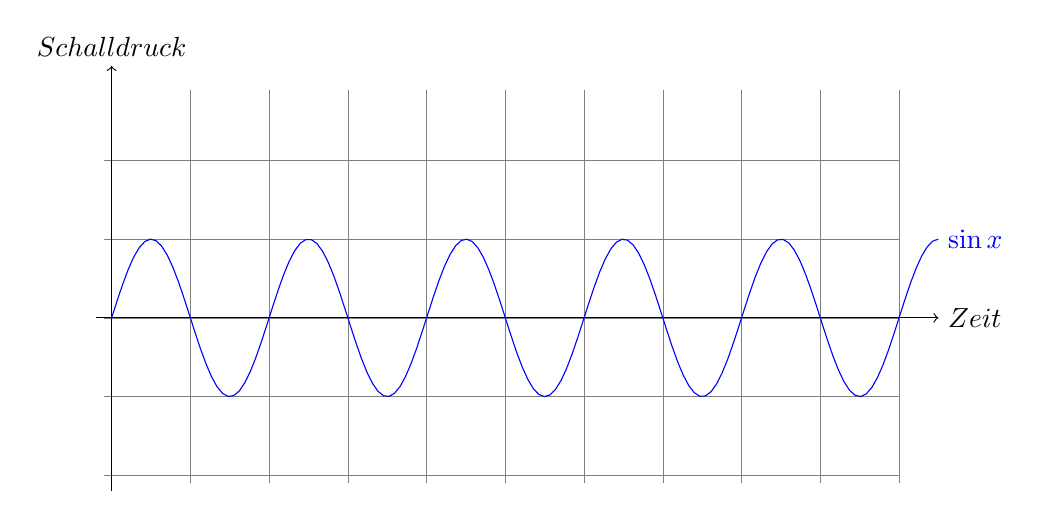
\begin{tikzpicture}[domain=0:10.5]
        \draw[very thin,color=gray] (-0.1,-2.1) grid (10,2.9);
        \draw[->] (-0.2,0) -- (10.5,0) node[right] {$Zeit$}; \draw[->] (0,-2.2) -- (0,3.2) node[above] {$Schalldruck$};
        % \draw[color=blue, samples=150]	plot (\x,{sin(\x r)})	node[right] {$f(x) = \sin x$};
        \draw[color=blue, samples=150]	plot (\x,{sin(pi*\x r)})	node[right] {$\sin x$};
    \end{tikzpicture}
    \caption{Wellenform eines Tons}
    \label{wav_sound}
\end{figure}
%

Anhand der Wellenform kann die Frequenz eines Tons abgeleitet und in Hertz (kurz: hz) angegeben werden. Die Frequenz gibt die Anzahl an Zyklen des Tons pro Sekunde an. Wenn beispielsweise \cref{wav_sound} eine Sekunde darstellt, entspricht die Frequenz 5hz, da sie fünf symmetrische Wellen aufweißt.

\par

Diese Vibration kann durch unterschiedliche Gegenstände erzeugt werden. Dazu zählen Becken eines Schlagzeugs, Saiten eines Kontrabasses oder die Stimmbänder einer Person. In diesem Projekt werden die Perkussionsinstrumente von den restlichen Instrumenten einer Wav-Datei getrennt.

\par

Bei der Darstellung mehrerer Signale werden einzelne Signale zu einer gemeinsamen Wellenform addiert.
In \cref{wav_multiple_sounds} werden eine 5hz (rot) und eine 2,5hz (blau) Wellenform gleichzeitig aufgenommen.
Der Summe der beiden Signale (grün) sind die einzelnen Bestandteile kaum abzulesen.
Die Herausforderung Frequenzen der Bestandteile zu identifizieren wird mittels Transformationen bewältigt.

%
\begin{figure}[h]
    \centering
    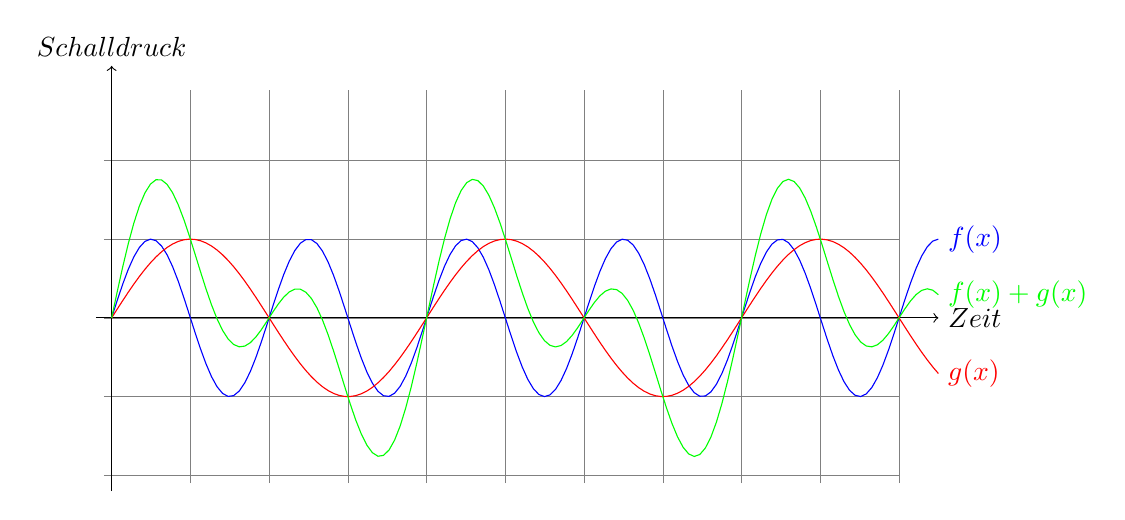
\begin{tikzpicture}[domain=0:10.5]
        \draw[very thin,color=gray] (-0.1,-2.1) grid (10,2.9);
        \draw[->] (-0.2,0) -- (10.5,0) node[right] {$Zeit$}; \draw[->] (0,-2.2) -- (0,3.2) node[above] {$Schalldruck$};
        % \draw[color=blue, samples=150]	plot (\x,{sin(\x r)})	node[right] {$f(x) = \sin x$};
        \draw[color=blue, samples=150]	plot (\x,{sin(pi*\x r)})	node[right] {$f(x)$};
        \draw[color=red, samples=150]	plot (\x,{sin(pi*\x r / 2)})	node[right] {$g(x)$};
        \draw[color=green, samples=150]	plot (\x,{sin(pi*\x r / 2) + (sin(pi*\x r))})	node[right] {$f(x) + g(x)$};
    \end{tikzpicture}
    \caption{Wellenform eines Tons}
    \label{wav_multiple_sounds}
\end{figure}
%

%
\section{Musikinstrumentgruppen}
\label{instrument_groups}
%

Musikinstrumente können in mehrere Gruppen aufgeteilt werden.
Diese unterscheiden sich voneinander in der Entstehung und dem Klang der Töne.
In diesem Projekt werden akkustische Instrumente behandelt, die in harmonische und perkussive Instrumente aufgeteilt werden.
Darüberhinaus existieren noch elektrische und digitale Instrumente.
Sie benötigen entweder Elektrizität oder einen Computerprozessor, um wie vorgesehen zu funktionieren.
Allerdings werden sie in diesem Projekt nicht behandelt.

\subsection{Behandelte Instrumentgruppen}

\textbf{Akkustische Instrumente} erzeugen einen Ton indem Menschen Kraft auf sie ausüben.
Sie benötigen keinen Strom, keine Verstärkung und keinen Computerprozessor, um einen Ton zu erzeugen und sind die ältesten Instrumente.
Sie können in perkussive und harmonische Instrumente unterteilt werden. 

\par

\textbf{Perkussive Instrumente} werden geschlagen, geschüttelt oder geschabt und sind eine spezielle Form der akkustischen Instrumente.
Die übrigen akkustischen Instrumente sind \textbf{harmonisch} \parencite{acoustic_electric_digital_instruments}.
In diesem Projekt wird versucht perkussive und harmonische Instrumente zu trennen.

%
\subsection{Vorteile der Instrumentgruppen für die Signalverarbeitung}
%

Akkustische Musikinstrumente zeichnet deren natürliche Entstehung aus. Bei der Entstehung von Tönen werden zusammenhängende Schallwellen erzeugt, deren Verlauf kontinuierlich ist. Dadurch werden akkustische Instrumente effektiver voneinander getrennt, da deren Verlauf nachvollziehbar ist.

\par

Zudem sind perkussive und harmonische Musikinstrumente geeignet für die Trennung voneinander. Die unterschiedlichen Signale zeichnen sich durch die Extreme der Ausschläge der Frequenzen aus. Während perkussive Instrumente bei der Entstehung einen deutlichen Ausschlag aufweisen, verlaufen harmonische Instrumente einheitlich mit weniger extremen Ausschlägen (siehe Vergleich von \cref{fig:percussive_analysis} und \cref{fig:harmonic_analysis}).

%
\section{Formen der Musikdarstellungen}
%

Musik kann unterschiedlich dargestellt werden und es wird je nach Bedarf eine andere Form der Musikdarstellung benötigt. Unterteilt wird in Musiknoten, symbolische Darstellungen und Audiodarstellungen.

%
\subsection{Musiknoten und symbolische Darstellung}
%

Musiknoten sind eine formale Sprache, die vorgibt wie ein Musikstück gespielt wird \parencite{sheet_music_representations}.
Bei symbolischen Darstellungen werden eindeutige Entitäten definiert, die von einem Computer übersetzt werden.
Beispielsweise wird der Musical Instrument Digital Interface (kurz: MIDI) Standard verwendet, um Informationen eines gespielten Tons möglichst detailliert zu speichern und abzurufen.

\subsection{Audiodarstellung}

Eine weitere Form der Darstellung, ist die Audiodarstellung. In dieser Darstellung werden die Informationen von Tönen als Audiosignale digital gespeichert und geteilt. Es werden die Schallwellen eines Tons (siehe \cref{sounds}) aufgenommen und digital als eine Wellenform gespeichert, die an der Schallwelle orientiert ist. Dazu gehören auch das Timing, die Intensität, die Lautstärke, die Länge des Tons und vieles mehr. Es werden nicht die einzelnen Töne und Noten gespeichert, sondern die Frequenzen während der Aufnahme in Abhängigkeit zur Zeit. Die Audiodatei kann auch Nebengeräusche oder weitere Instrumente beinhalten (\cite{fundamentals_of_music_processing}, S. 1ff).

%
\subsection{Einordnung in den Projektkontext}
%

Bei der Trennung von Musikinstrumenten wird aufgenommene Musik in der digitalen Darstellung behandelt. Diese Darstellung erschwert es unterschiedliche Audiosignale zu trennen und deren ursprüngliche Töne zu reproduzieren, dessen verbreitetste Darstellungsform MP3 ist \parencite{mp3_most_popular}. In diesem Projekt werden jedoch Wav-Dateien behandelt. Die Unterschiede, sowie Vor- und Nachteile der Audiodarstellungen werden in \cref{audio_representations} behandelt.

%
\section{Aufbau einer Audiodatei}
%

Für die Aufnahme von Audiosignalen werden analoge Signale in eine digitale Form von Schall umgewandelt. Ein analoges Signal basiert auf kontinuierlichen und konstanten Spannungsschwankungen, die den verursachten Luftdruckschwankungen entsprechen \parencite{digital_representation}. In der digitalen Form werden die Spannungsschwankungen als Bitstreams gespeichert und je nach Audio-Format komprimiert.

%
\subsection{Durchführung der Komprimierung}
\label{compression}
%

Die Komprimierung von Audiodateien wird meistens verwendet, um mehr Musik auf einem Datenträger speichern zu können \parencite{what_is_audio_compression}. Für die Komprimierung einer Aufnahme wird diese in eine Samplingrate (auch: Abtastrate) und eine Quantisierungsschrittweite reduziert.

%
\textbf{Samplingrate}
%

Die Samplingrate definiert die Anzahl von gespeicherten Signalen pro Sekunde.
Dies reduziert die benötigten gespeicherten Daten einer durchgängigen Aufnahme auf mehrere Blöcke (siehe: \cref{fig:samplingrate}).
Beispielsweise werden auf einer CD 44.100 Werte pro Sekunde gespeichert (kurz: 44.1 kHz), dessen Übergänge kaum wahrnehmbar sind, jedoch bereits zu einer deutlichen Reduzierung des Speicherbedarfs führen.

%
\textbf{Quantisierungsschrittweite}
%

Die Quantisierungsschrittweite beschreibt die Auflösung, mit der jedes Sample komprimiert wird.
Die möglichen Werte eines Samples sind kontinuierlich und könnten theoretisch unendlich viele Dezimalstellen haben.
Durch die Quantisierungsschrittweite werden diese Werte auf eine festgelegte Anzahl möglicher diskreter Werte reduziert, wodurch der Unterschied zwischen den Werten bestimmt wird.
Bei CDs wird beispielsweise eine 16-Bit-Codierung gewählt, die 65.536 mögliche Werte definiert.

%
\begin{figure}[h]
    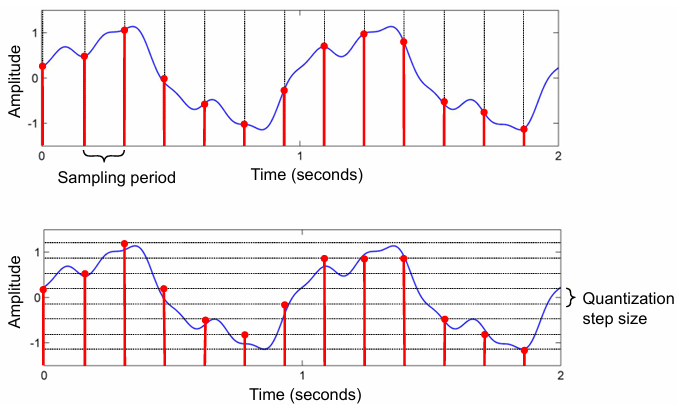
\includegraphics[width=1\textwidth]{images/Samplingrate_Quantisierungsgröße.PNG}
    \caption[Unterteilung in Samplingrate und Quantisierungsschrittweite]{Unterteilung in Samplingrate (oben) und Quantisierungsschrittweite\\\hspace{\textwidth}\textit{Quelle}: \cite{fundamentals_of_music_processing}, S. 61}
    \label{fig:samplingrate}
\end{figure}
%

%
\subsection{Waveform Audio File Format}
%

Das Waveform Audio File Format (kurz: Wav-Datei) speichert Audioaufnahmen unkomprimiert \parencite{what_is_a_wav_file}. Der Begriff leitet sich \enquote{vom englischen Wort \enquote{wave}} \parencite{wav} für Schallwelle ab. Für die in diesem Projekt behandelte Fourier Transform sind insbesondere die \enquote{Abtastrate fs des Messsystems} und die Quantisierungsschrittweite (siehe \cref{compression}) entscheidend  \parencite{FFT_grundlagen}. Aufgrund der unkomprimierten Speicherung (und der damit verbundenen hohen Abtastrate und Quantisierungsschrittweite) lässt sich eine klare Trennung von Tonspuren ermöglichen.


%
\subsection{Andere Formen von Audio-Dateien}
\label{audio_representations}
%

Außer Wav-Dateien gibt es noch einige weitere verbreitete Speicherformate für Audio. Jede dieser Speicherformen hat Vor- und Nachteile und eigene Anwendungsszenarien. Allerdings stellt sich heraus, dass keine Speicherform einen geringeren Informationsverlust als Wav-Dateien aufweist.

%
\begin{itemize}
    \item [MP3:] Verwendet standardisiertes Komprimierungsverfahren und benötigt relativ wenig Speicherplatz bei vergleichsweise hoher Qualität.
    \item [WMA:] Speziell für Microsoft entwickeltes Dateiformat ebenfalls mit sowohl hoher Kompression als auch guter Qualität.
    \item [AAC:] Ist eine Weiterentwicklung der Entwickler:innen von MP3 mit verbessertem Verhältnis aus Komprimierung und Qualität.
    \item [OGG:] Wurde als frei-verfügbare Alternative zu MP3 entwickelt.
    \item [FLAC:] Steht ebenfalls patentfrei zur Verfügung und implementiert ein Verfahren zum Kodieren und Dekodieren der Daten.
    \item [RM:] Steht für Real Media und beinhaltet as Real Audio Format mit Fokus auf guter Qualität, trotz Komprimierung.
\end{itemize}
%

\parencite{audioformate_im_überblick}

%
\section{Trennung einer Tonspur in verschiedene Instrumente}
%

Eine Aufnahme speichert das eingehende Signal in Abhängigkeit zur Zeit. Dabei weist jedes Signal charakteristische Schwingungen in Form einer Wellenform auf. Während einer Aufnahme überlagern sich mehrere Signale zu einer gemeinsamen Wellenform, was ihre Unterscheidung erschwert (siehe: \cref{wav_multiple_sounds}). Dies tritt insbesondere bei Hintergrundgeräuschen oder bei der parallelen Aufnahme mehrerer Musikinstrumente auf.

\par

Die Trennung von Signalen ist ein Thema, das in Forschung und Bildung intensiv behandelt wird (siehe: \cref{stand_der_wissenschaft}). Eine der am häufigsten verwendete Methode ist die Fourier Transform (\cite{fundamentals_of_music_processing}, S.39), die es ermöglicht, ein Signal in seine Frequenzkomponenten zu zerlegen. Diese wird auch bei der Audioverarbeitung für die Trennung von Instrumenten innerhalb einer Tonspur verwendet.

\par

Neben der Fourier Transform werden weitere Ansätze wie die Wavelet Transform, die Short-Time Fourier Transform (kurz: STFT), sowie statistische Verfahren wie die Blind Source Separation (BSS) und die Independent Component Analysis (ICA) eingesetzt. Darüber hinaus finden moderne Verfahren des maschinellen Lernens, insbesondere neuronale Netzwerke, zunehmend Anwendung in der Trennung von Audiosignalen.

%
\subsection{Fourier Transform}
%

Die Fourier Transform ist ein Algorithmus der die Darstellung einer Tondatei verändert. Ursprünglich liegt die Audiospur mit einer Kombination aus unterschiedlichen Frequenzen in Abhängigkeit zur Zeit vor. In dieser Darstellung sind die unterschiedlichen Signale schwierig zu trennen und werden von der Fourier Transform transformiert.

\par

%
\subsubsection{Entwicklung der Fourier Transform}
%

Die Fourier Transform ist eine Verallgemeinerung der Fourierreihen. Diese Reihen können stetige oder stückweise stetige Funktionen in eine Summe von Sinus- und Kosinusfunktionen zerlegen. Bereits im 18. Jahrhundert wurden Fourierreihen für spezifische Funktionen entdeckt. 1822 stellte Joseph Fourier die Hypothese auf, dass sich jede Funktion als Summe solcher Reihen darstellen lässt.

\par

Erst im 20. Jahrhundert wurden Fourierreihen auch für andere stetige oder stückweise stetige Funktionen formal bewiesen. Dank der Vollständigkeit der Funktionenreihe lässt sich die Fourier Transform auf eine Vielzahl von Funktionen anwenden, einschließlich periodischer und nicht-periodischer Funktionen, und erhielt ihren Namen zu Ehren von Joseph Fourier.

%
\subsubsection{Durchführung der Transformation}
%

Die Fourier Transform ist ein mathematisches Verfahren, bei dem ein Signal aus dem Zeitbereich in den Frequenzbereich transformiert wird (siehe: \cref{fig:frequency_to_time}). Die Transformation ermöglicht es, beliebige periodische und stückweise stetige Funktionen als Summe von Sinus- und Kosinuswellen unterschiedlicher Frequenzen darzustellen.

\par

In der neuen Darstellung werden die Frequenzen der Funktion unabhängig von der zeitlichen Komponente wiedergegeben. Unterschiedliche Frequenzen können unterschiedlichen Signalen zugeordnet werden. Die frequentielle Darstellung gibt an welche Signale in welchen Frequenzen Teil der Funktion sind, allerdings nicht wann. Daher wird die Darstellung wieder zurückgeformt in die zeitliche Abhängigkeit.

\par

Das Signal oder die Signale, die von der Tonspur getrennt werden, können in der frequentiellen Darstellung identifiziert werden. Anschließend werden diese von den übrigen Signalen getrennt und zurück in die ursprüngliche Darstellung transformiert (Inverse Fourier Transform). Damit erhält man eine neue Tondatei, die ausschließlich aus den benötigten Signalen besteht.

% \subsubsection{Parameter der Transformation}

%  - Probleme:
%     - Rechenaufwand/ Dauer

% In \cref{compression} wurden die relevanten Parameter wie Samplingrate und Quantisierungsschrittweite behandelt, die für die Durchführbarkeit der Transformation entscheidend sind. Zudem können verschiedene Komponenten der Transformation konfiguriert bzw. parametrisiert werden.

% \par

% %
% \textbf{Blocklänge (/engl.?)}
% %

% Ein wesentlicher Parameter für die Durchführung der Fourier Transform ist die Blocklänge (kurz: BL), welche die Anzahl der Samples festlegt, die in der Fourier Transform analysiert werden.

% \par

% Umso länger die BL, desto präziser ist das Ergebnis der Transformation. Dies erhöht jedoch auch den Rechenaufwand und die Dauer der Transformation. In einigen Anwendungsszenarien erfordert dies eine Abwägung zwischen Verarbeitungsdauer und Genauigkeit, beispielsweise in einer App zum Stimmen von Musikinstrumenten oder zum Erkennen der gespielten Töne (Quelle?).

%
\begin{figure}[h]
    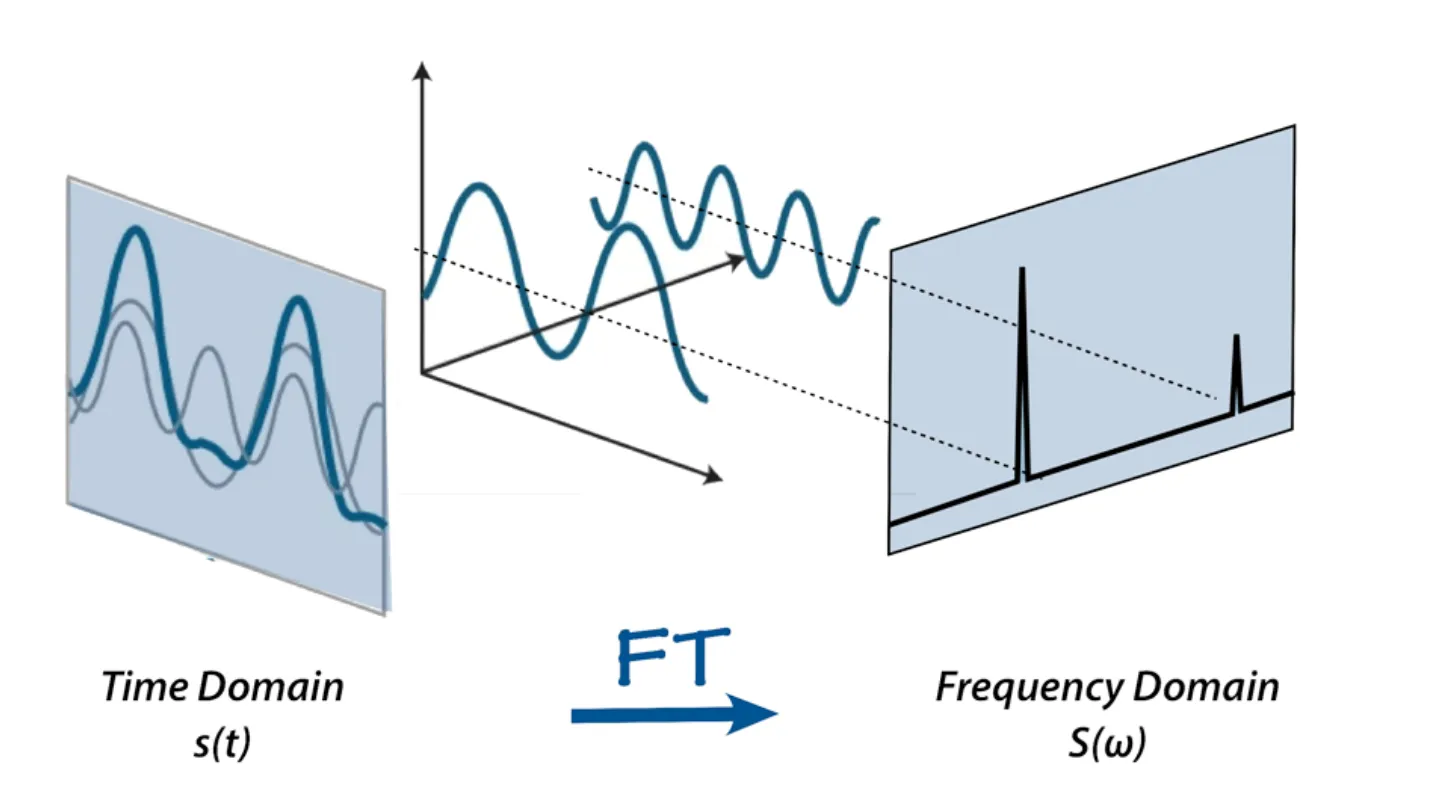
\includegraphics[width=1\textwidth]{time_to_frequency_domain.png}
    \caption[Transformation von zeitlicher zu frequenzieller Darstellung]{Transformation von zeitlicher zu frequenzieller Darstellung\\\hspace{\textwidth}\textit{Quelle}: \cite{music_extraction}}
    \label{fig:frequency_to_time}
\end{figure}
%

\subsubsection{Durchführung am Beispiel einer Musiknote}

In diesem Beispiel (aus \cite{fundamentals_of_music_processing}, S.40f) wird eine Note auf einem Piano gespielt und durch die Transformation in eine frequentielle Darstellung umgeformt, in der ein gespielter Ton erkannt wird.

\par

% Die Aufnahme des Tons ist in \cref{fig:fourier}(a) zu erkennen. Für die Transformation wird ein Ausschnitt von 10ms verwendet. Das entspricht der Blocklänge und reduziert den Rechenaufwand (referenzieren?).

Die Aufnahme des Tons ist in \cref{fig:fourier}(a) zu erkennen. Für die Transformation wird ein Ausschnitt von 10ms verwendet, um den Rechenaufwand zu reduzieren und den Vorgang beispielhaft zu verdeutlichen.

%
\begin{figure}[h]
    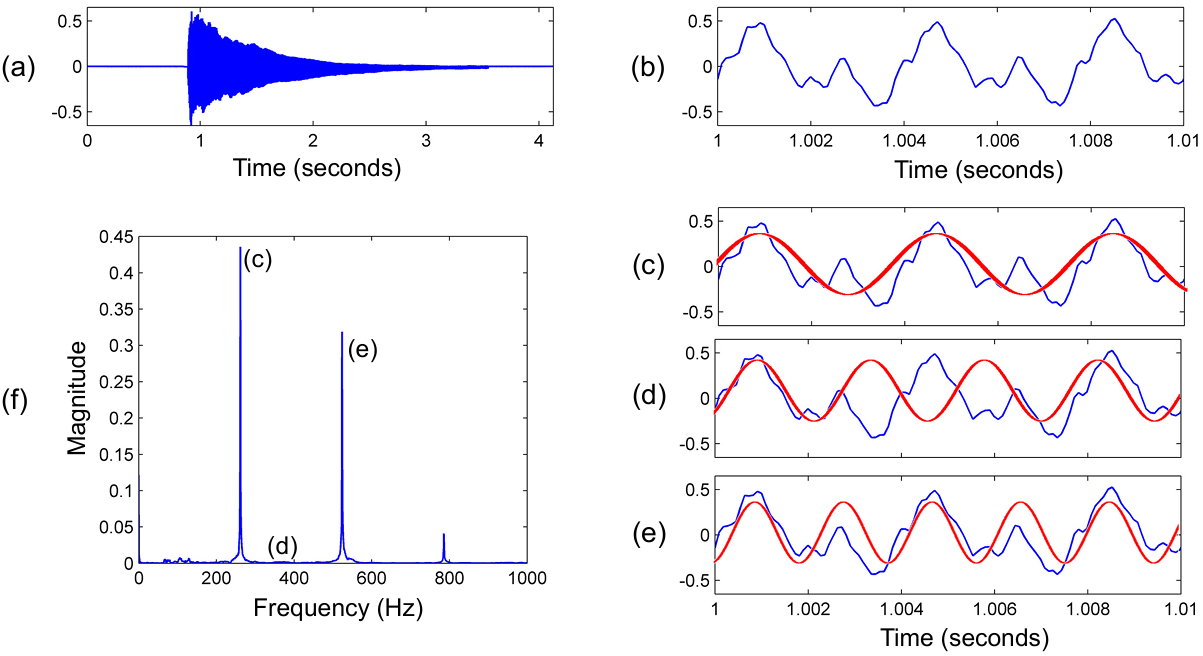
\includegraphics[width=1\textwidth]{images/Fourier_math.PNG}
    \caption[Note C4 in unterschiedlichen Darstellungen]{Note C4 in unterschiedlichen Darstellungen\\\hspace{\textwidth}\textit{Quelle}: \cite{fundamentals_of_music_processing}, S. 41}
    \label{fig:fourier}
\end{figure}
% Music Processing S.41
%

Anschließend werden unterschiedliche Vergleichsfunktionen für die jeweiligen Frequenzen mit dem Ausschnitt der Tonspur verglichen. Die Ähnlichkeiten der jeweiligen Frequenzen werden in (f) wiedergegeben.

\par

In \cref{fig:fourier}(c) ist die Übereinstimmung für die Frequenz w = 262 Hz besonders hoch. Daraus folgt in (f) bei ungefähr 262 der höchste Wert. Die Höhe des Wertes wird in der Variable dw angegeben.

% w = ω

\par

Die Frequenz 262 entspricht der Note C4. Darüberhinaus wird bei einer Frequenz von 523 (siehe \cref{fig:fourier}(e)) eine hohe Übereinstimmung erkannt. Dies entspricht ungefähr der Frequenz des zweiten Teiltons der Note C4.

%
\subsubsection{Nachteile der Fourier Transform}
\label{disadvantages_fourier}
%
    
Die Fourier Transform ermöglicht es je nach Bedarf zwischen der zeitlichen oder der sequentiellen Darstellung zu wechseln. Allerdings ist dieser Wechsel zwischen den Darstellung notwendig und es wird entweder die zeitliche oder die frequentielle Komponente ignoriert. Bei der Anwendung der Fourier Transform gibt es keine Darstellung die beide Komponenten kombiniert.

\par

Außerdem wird bei der Fourier Transform die ganze Datei bearbeitet. Dies führt bei größeren Dateien zu großem Rechenaufwand des Prozessors und zu Ungenauigkeiten in der Durchführung, da kleinere Abschnitte ignoriert werden.

%
\subsection{Wavelet Transform}
\label{wavelet-transformation}
%

Die Wavelet Transform ist ein Verfahren, das eine zeitliche Darstellung einer Funktion in eine dreidimensionale Darstellung in Abhhängigkeit von Zeit und Frequenz überführt. Dabei werden sogenannte Wavelets - spezielle Wellenfunktionen - mit der ursprünglichen Funktion verglichen, um Übereinstimmungen zu finden (siehe: \cref{wavelet_examples}). Der Begriff \enquote{Wavelet} stammt aus dem Französischen und bedeutet \enquote{kleine Welle} oder \enquote{Wellchen}.

%
\begin{figure}[h]
    \centering
    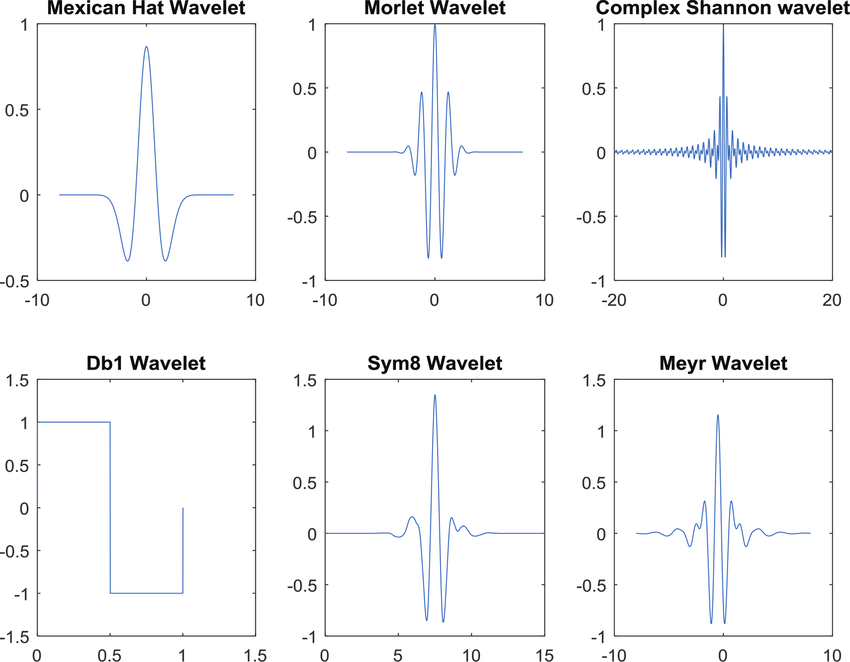
\includegraphics[width=0.7\textwidth]{wavelets.png}
    \caption[Wavelet Beispiele in zweidimensionaler Darstellung]{Wavelet Beispiele in zweidimensionaler Darstellung\\\hspace{\textwidth}\textit{Quelle}: \cite{wavelet_examples}}
    \label{fig:wavelet_examples}
\end{figure}
%

Im Gegensatz zur ursprünglichen Funktion haben die Wavelets eine endliche Fläche (auch: finite energy), was sie begrenzt und lokalisiert. Eine weitere Bedingung für Wavelets ist, dass ihr Integral null ergibt, d.h., dass die Fläche über und unter der X-Achse gleich groß ist (Admissibility condition). Unterschiedliche Wavelets verfügen über unterschiedliche Anwendungsszenarien.

\textbf{Jedes Wavelet wird durch die Parameter m und b ergänzt:}

%
\begin{itemize}
    \item[m:] Bestimmt die Frequenz des Wavelets
    \item[b:] Bestimmt den Zeitpunkt des Wavelets
\end{itemize}
%

Zudem besitzt das Wavelet einen realen und einen imaginären Teil. Durch die Berücksichtigung des imaginären Teils entsteht eine dreidimensionale Darstellung des Signals (siehe: \cref{fig:wavelet_transform}). Bei der Wavelet Transform wird sowohl der reale als auch der imaginäre Teil des Wavelets mit der Funktion korreliert (Mathematik: Korrelation), um die Ähnlichkeit der Funktion und des Wavelets zu berechnen. Diese Ähnlichkeit wird für jedes m und b ermittelt und in einem dreidimensionalen Ausgabe-Graphen in Abhängigkeit von der Zeit und der Frequenz dargestellt (siehe: \cite{wavelet_transform}).

%
\begin{figure}[h]
    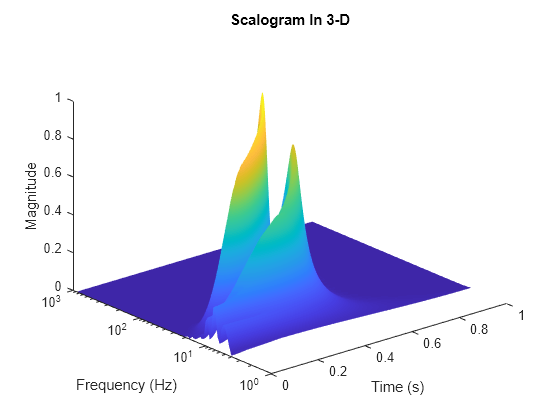
\includegraphics[width=1\textwidth,trim={0 0 0 2cm},clip]{wavelet_transform.png}
    \caption[Frequentielle und zeitliche Darstellung nach Wavelet Transform]{Frequentielle und zeitliche Darstellung nach Wavelet Transform\\\hspace{\textwidth}\textit{Quelle}: \cite{wavelet_transform}}
    \label{fig:wavelet_transform}
\end{figure}
%

Ein Anwendungsfall ist die Überprüfung von Ampelleuchten. Während die Fourier Transform die verschiedenen Frequenzen der Farben Grün, Gelb und Rot erkennt, um festzustellen, ob die Lampen leuchten, erlaubt die Wavelet Transform zusätzlich die Angabe, ob die Lichter zu den richtigen Zeitpunkten aufleuchten \parencite{wavelets}.

%
\subsection{Wahl der Fourier Transform}
%

Für die Trennug der Instrumente einer Wav-Datei wurde die Fourier Transform gewählt, trotz einiger Alternativen. Die Fourier Transform ist eines der meistverwendeten Werkzeuge der Signalverarbeitung (\cite{fundamentals_of_music_processing}, S.39). Der größte Nachteil der Fourier Transform ist, dass nicht gleichzeitig die Zeit und die Frequenz Domäne dargestellt werden können.

\par

Jedoch reicht dies bei der Trennung von Musikinstrumenten, da die Darstellung zum Schluss wieder in die zeitliche Domäne umgeformt wird, um das Ergebnis in eine Wav-Datei zu überführen. Außerdem verliert die Fourier Transform wenig Informationen durch die klare Trennung von zeitlicher und frequentieller Darstellung \parencite{Parsons_2000}.

\par

Allerdings ist die Fourier Transform bei größeren Dateien aufwändiger und fehleranfälliger, falls die ganze Datei transformiert wird. Jedoch wird diese Limitierung durch die Verwendung der Short-Time Fourier Transform reduziert \parencite{Prashanth_2017}.

%
\subsection{Short-Time Fourier Transform}
%

Die Short-Time Fourier Transform (auch: STFT) basiert auf der Fourier Transform, dessen Nachteile zunehmender Aufwand und fehleranfälligkeit bei der Transformation größerer Dateien beihaltet (siehe: \cref{disadvantages_fourier}). Damit ist es eins der wichtigsten Tools in der Audioverarbeitung (\cite{fundamentals_of_music_processing}, S.110).

\par

Stattdessen teilt die STFT eine Datei in mehrere kleine Pakete, deren Transformation effizienter und effektiver durchgeführt werden können. Anschließend werden die Übergänge der Pakete geglättet, um Unregelmäßigkeiten zu vermeiden. In \cref{stft_code} wird die praktische Umsetzung mittels Programmcode dargestellt und die Funktionalität erläutert.